%% Time-stamp: <2019-01-15 14:22:02 (marc)>
\documentclass[xcolor=x11names,compress, mathserif]{beamer}

\newcommand\hmmax{0}
\newcommand\bmmax{0}

\usepackage{../includes/MarkMathCmds}

\newcommand{\hackspace}{\hspace{4.2mm}}
\newcommand{\showstudent}[1]{}





% talk/author information
\newcommand{\authorname}{Mark van der Wilk}
\newcommand{\authoremail}{m.vdwilk@imperial.ac.uk}
\newcommand{\authoraffiliation}{
 Department of Computing\\Imperial
  College London}
\newcommand{\authortwitter}{markvanderwilk}
\newcommand{\slidesettitle}{\imperialBlue{Graphical Models}}
\newcommand{\footertitle}{Graphical Models}
\newcommand{\location}{Imperial College London}
\newcommand{\talkDate}{{January 16, 2022}}



\date{\imperialGray{\talkDate}}




% load defaults
\selectcolormodel{rgb}
\usepackage{ifxetex,ifluatex}
\newif\ifxetexorluatex
\ifxetex
  \xetexorluatextrue
\else
  \ifluatex
    \xetexorluatextrue
  \else
    \xetexorluatexfalse
  \fi
\fi

\usepackage{textpos}
%\usepackage{arabtex}
\usepackage{tikz}
\usetikzlibrary{decorations.markings}
\usetikzlibrary{arrows}
\usetikzlibrary{shapes}
\usetikzlibrary{plotmarks}
\usetikzlibrary{mindmap,trees,backgrounds}

\tikzstyle{every picture}+=[remember picture]

%\usepackage{movie15}
% \usepackage{pdfpages}
%\usepackage{xmpmulti}

\usepackage{anyfontsize}
\usepackage{wrapfig}
\usepackage{animate}
\usepackage{multirow}
\usepackage{multimedia}
\usepackage{xmpmulti}
%\usepackage[latin9]{inputenc}
\usepackage[english]{babel}
\usepackage{scalefnt}
\usepackage{verbatim}
\usepackage{url}
% \usepackage{pgf,pgfarrows,pgfnodes}
\usepackage{textpos}
\usepackage[tight,ugly]{units}
\usepackage{url}
\usepackage{bbm}
\usepackage[english]{babel}
\usepackage{fancyhdr}
\usepackage{bm} % correct bold symbols, like \bm
\usepackage{amsmath}
\usepackage{amsfonts}
\usepackage{amssymb}
\usepackage{mathrsfs}
\usepackage{mathtools}
\usepackage{color}
\usepackage{cancel}
\usepackage{algorithm}
\usepackage{algpseudocode}
\usepackage{mathrsfs}
\usepackage{listings}
\usepackage{graphicx} % for pdf, bitmapped graphics files
\usepackage{mathtools}
\usepackage{units}
\usepackage{subfig}
\usepackage{enumerate}
\usepackage{natbib}
\usepackage{dsfont}


\ifxetexorluatex
\usepackage{fontspec}
\setmainfont[Scale=0.8]{OpenDyslexic-Regular}
\else
\usefonttheme{professionalfonts}
\fi

\renewcommand{\vec}[1]{{\boldsymbol{{#1}}}} % vector
\newcommand{\mat}[1]{{\boldsymbol{{#1}}}} % matrix
% \newcommand{\KL}[2]{\mathrm{KL}(#1\|#2)} % KL divergence
\newcommand{\R}[0]{\mathds{R}} % real numbers
\newcommand{\Z}[0]{\mathds{Z}} % integers
\newcommand{\tr}[0]{\text{tr}} % trace
% \newcommand{\inv}{^{-1}}
% \DeclareMathOperator*{\diag}{diag}
\newcommand{\E}{\mathds{E}} % expectation
\newcommand{\var}{\mathds{V}}
\newcommand{\gauss}[2]{\mathcal{N}\big(#1,\,#2\big)}
\newcommand{\gaussx}[3]{\mathcal{N}\big(#1\,|\,#2,\,#3\big)}
\newcommand{\gaussBig}[2]{\mathcal{N}\left(#1,\,#2\right)}
\newcommand{\gaussxBig}[3]{\mathcal{N}\left(#1\,\left|\,#2,\,#3\right.\right)}
\newcommand{\Ber}[0]{\mathrm{Ber}} % Bernoulli distribution
\DeclareMathOperator{\cov}{Cov}
\ifxetexorluatex
\renewcommand{\T}[0]{^\top}
\renewcommand{\d}[0]{\text{d}} % derivative
\else
\newcommand{\T}[0]{^\top}
\renewcommand{\d}[0]{\text{d}} % derivative
\fi
% calculus
\newcommand{\pdiff}[1]{\frac{\partial}{\partial #1}}
\newcommand{\pdiffF}[2]{\frac{\partial #1}{\partial #2}}
\newcommand{\diffF}[2]{\frac{{\d}#1}{{\d}#2}}
\newcommand{\diffFII}[2]{\frac{{\d}^2 #1}{{\d}#2^2}}
\newcommand{\diff}[1]{\frac{{\d}}{{\d}#1}}
\newcommand{\diffII}[1]{\frac{{\d}^2}{{\d}#1^2}}
\newcommand{\class}[0]{\mathcal{C}}

\newcommand{\idx}[1]{^{(#1)}}
% \newcommand{\norm}[1]{\left\|#1\right\|}
\newcommand{\proj}[1]{\tilde{#1}}
\newcommand{\pcacoord}{z}
\newcommand{\pcacoordnew}{\zeta}
\newcommand{\latent}{z}
% \newcommand{\given}{\,|\,}
\newcommand{\genset}[1]{\mathrm{span}[#1]} % generating set
\newcommand{\set}[1]{\mathcal{#1}} % set
\newcommand{\fixgmfont}[1]{\scalebox{0.8}{#1}}



\usepackage{pifont}% http://ctan.org/pkg/pifont
\newcommand{\cmark}{{\color{green!40!black}\ding{51}}}%
\newcommand{\xmark}{{\color{red}\ding{55}}}%
\newcommand{\green}[1]{{\bf{\textcolor{green}{#1}}}}
\newcommand{\red}[1]{{\bf{\textcolor{red}{#1}}}}

\newcommand<>\red[1]{{\color#2[rgb]{1,0,0}#1}}
\newcommand<>\blue[1]{{\color#2[rgb]{0,0,1}#1}}
\newcommand<>\yellow[1]{{\color#2{camyellow}#1}}
\newcommand<>\green[1]{{\color#2[rgb]{0,0.6,0.0}#1}}
\newcommand<>\violet[1]{{\color#2[rgb]{0.6,0,0.6}#1}}
\newcommand<>\orange[1]{{\color#2[rgb]{1,0.5,0}#1}}
\newcommand<>\black[1]{{\color#2[rgb]{0,0,0}#1}}
\newcommand<>\steel[1]{{\color#2[rgb]{0,0,0.8}#1}}
\newcommand<>\darkblue[1]{{\color#2[rgb]{0,0,0.6}#1}}
\newcommand<>\lightblue[1]{{\color#2[rgb]{0.4,0.4,0.7}#1}}
\newcommand<>\gray[1]{{\color#2[rgb]{0.4,0.4,0.4}#1}}
\newcommand<>\greenish[1]{{\color#2[rgb]{0.45, 0.66, 0.45}#1}}
\newcommand<>\redish[1]{{\color#2[rgb]{0.7843    0.3706    0.3706}#1}}
\definecolor{redishTIKZ}{rgb}{0.7843, 0.3706, 0.3706}
\definecolor{imperialBlue}{rgb}{0.058, 0.219, 0.418}
\definecolor{aimsbrown}{rgb}{0.539, 0.117, 0.015}
% \definecolor{imperialGray}{rgb}{0.414, 0.488, 0.671 }
\definecolor{imperialGray}{RGB}{109,153, 204}
\definecolor{aimslightbrown}{RGB}{138,88,84}
\newcommand<>\imperialBlue[1]{{\color#2[rgb]{0.058, 0.219, 0.418}#1}}
\newcommand<>\aimsbrown[1]{{\color#2[rgb]{0.539, 0.117, 0.015}#1}}
%\newcommand<>\imperialGray[1]{{\color#2[rgb]{0.414, 0.488, 0.671}#1}}
\newcommand<>\imperialGray[1]{{\color#2[RGB]{109,153, 204}#1}}
\newcommand<>\aimslightbrown[1]{{\color#2[RGB]{138,88,84}#1}}
\newcommand<>\lightgray[1]{{\color#2[rgb]{0.8,0.8,0.8}#1}}
%\newcommand<>\highlightcolor[1]{{\color#2[rgb]{0,0,1}#1}}
\newcommand{\highlight}[1]{{\bf\steel{#1}}}
%\newcommand{\newblock}[0]{}

%\newcommand{\arrow}[0]{\includegraphics[height=5pt]{./figures/arrow}\hspace{3pt}}

\renewcommand{\emph}[1]{\textbf{\steel{{#1}}}}

\renewcommand{\alert}[1]{{\bf\red{{#1}}}}

\newcommand{\arrow}{
\begin{tikzpicture}
\draw [black!40!green, fill=black!40!green] (0,-0.12) -- (0,0.12) --
(0.15,0);
\draw [black!40!green, fill=black!40!green] (0.15,-0.12) -- (0.15,0.12) --
(0.3,0); 
\end{tikzpicture}
}

\geometry{left=0.45cm,top=0cm,right=0.45cm}


\newcommand{\logoimagepath}{./figures/imperial}
\newcommand{\highlightcolor}{blue!80!black}
%\newcommand{\headbarcolor}{imperialBlue}
\newcommand{\headbarcolor}{imperialBlue}
\institute{}

\newcommand{\coursetitle}{}

\newcommand{\slidesetsubtitle}{}
\newcommand{\slidesetnumber}{01}
\usefonttheme{professionalfonts}


\usetikzlibrary{decorations.fractals}
% tikzlibrary.code.tex
%
% Copyright 2010-2011 by Laura Dietz
% Copyright 2012 by Jaakko Luttinen
%
% The MIT License
%
% See LICENSE file for more details.

% Load other libraries
\usetikzlibrary{shapes}
\usetikzlibrary{fit}
\usetikzlibrary{chains}
\usetikzlibrary{arrows}

% Latent node
\tikzstyle{latent} = [circle,fill=white,draw=black,inner sep=1pt,
minimum size=20pt, font=\fontsize{10}{10}\selectfont, node distance=1]
% Observed node
\tikzstyle{obs} = [latent,fill=gray!25]
% Constant node
\tikzstyle{const} = [rectangle, inner sep=0pt, node distance=1]
% Factor node
\tikzstyle{factor} = [rectangle, fill=black,minimum size=5pt, inner
sep=0pt, node distance=0.4]
% Deterministic node
\tikzstyle{det} = [latent, diamond]

% Plate node
\tikzstyle{plate} = [draw, rectangle, rounded corners, fit=#1]
% Invisible wrapper node
\tikzstyle{wrap} = [inner sep=0pt, fit=#1]
% Gate
\tikzstyle{gate} = [draw, rectangle, dashed, fit=#1]

% Caption node
\tikzstyle{caption} = [font=\footnotesize, node distance=0] %
\tikzstyle{plate caption} = [caption, node distance=0, inner sep=0pt,
below left=5pt and 0pt of #1.south east] %
\tikzstyle{factor caption} = [caption] %
\tikzstyle{every label} += [caption] %

%\pgfdeclarelayer{b}
%\pgfdeclarelayer{f}
%\pgfsetlayers{b,main,f}

% \factoredge [options] {inputs} {factors} {outputs}
\newcommand{\factoredge}[4][]{ %
  % Connect all nodes #2 to all nodes #4 via all factors #3.
  \foreach \f in {#3} { %
    \foreach \x in {#2} { %
      \path (\x) edge[-,#1] (\f) ; %
      %\draw[-,#1] (\x) edge[-] (\f) ; %
    } ;
    \foreach \y in {#4} { %
      \path (\f) edge[->, >={triangle 45}, #1] (\y) ; %
      %\draw[->,#1] (\f) -- (\y) ; %
    } ;
  } ;
}

% \edge [options] {inputs} {outputs}
\newcommand{\edge}[3][]{ %
  % Connect all nodes #2 to all nodes #3.
  \foreach \x in {#2} { %
    \foreach \y in {#3} { %
      \path (\x) edge [->, >={triangle 45}, #1] (\y) ;%
      %\draw[->,#1] (\x) -- (\y) ;%
    } ;
  } ;
}

% \factor [options] {name} {caption} {inputs} {outputs}
\newcommand{\factor}[5][]{ %
  % Draw the factor node. Use alias to allow empty names.
  \node[factor, label={[name=#2-caption]#3}, name=#2, #1,
  alias=#2-alias] {} ; %
  % Connect all inputs to outputs via this factor
  \factoredge {#4} {#2-alias} {#5} ; %
}

% \plate [options] {name} {fitlist} {caption}
\newcommand{\plate}[4][]{ %
  \node[wrap=#3] (#2-wrap) {}; %
  \node[plate caption=#2-wrap] (#2-caption) {#4}; %
  \node[plate=(#2-wrap)(#2-caption), #1] (#2) {}; %
}

% \gate [options] {name} {fitlist} {inputs}
\newcommand{\gate}[4][]{ %
  \node[gate=#3, name=#2, #1, alias=#2-alias] {}; %
  \foreach \x in {#4} { %
    \draw [-*,thick] (\x) -- (#2-alias); %
  } ;%
}

% \vgate {name} {fitlist-left} {caption-left} {fitlist-right}
% {caption-right} {inputs}
\newcommand{\vgate}[6]{ %
  % Wrap the left and right parts
  \node[wrap=#2] (#1-left) {}; %
  \node[wrap=#4] (#1-right) {}; %
  % Draw the gate
  \node[gate=(#1-left)(#1-right)] (#1) {}; %
  % Add captions
  \node[caption, below left=of #1.north ] (#1-left-caption)
  {#3}; %
  \node[caption, below right=of #1.north ] (#1-right-caption)
  {#5}; %
  % Draw middle separation
  \draw [-, dashed] (#1.north) -- (#1.south); %
  % Draw inputs
  \foreach \x in {#6} { %
    \draw [-*,thick] (\x) -- (#1); %
  } ;%
}

% \hgate {name} {fitlist-top} {caption-top} {fitlist-bottom}
% {caption-bottom} {inputs}
\newcommand{\hgate}[6]{ %
  % Wrap the left and right parts
  \node[wrap=#2] (#1-top) {}; %
  \node[wrap=#4] (#1-bottom) {}; %
  % Draw the gate
  \node[gate=(#1-top)(#1-bottom)] (#1) {}; %
  % Add captions
  \node[caption, above right=of #1.west ] (#1-top-caption)
  {#3}; %
  \node[caption, below right=of #1.west ] (#1-bottom-caption)
  {#5}; %
  % Draw middle separation
  \draw [-, dashed] (#1.west) -- (#1.east); %
  % Draw inputs
  \foreach \x in {#6} { %
    \draw [-*,thick] (\x) -- (#1); %
  } ;%
}


% Copyright (C) 2016  Joseph Rabinoff

% ipe2tikz is free software; you can redistribute it and/or modify it under
% the terms of the GNU General Public License as published by the Free
% Software Foundation; either version 3 of the License, or (at your option)
% any later version.

% ipe2tikz is distributed in the hope that it will be useful, but WITHOUT ANY
% WARRANTY; without even the implied warranty of MERCHANTABILITY or FITNESS
% FOR A PARTICULAR PURPOSE.  See the GNU General Public License for more
% details.

% You should have received a copy of the GNU General Public License along with
% ipe2tikz; if not, you can find it at "http://www.gnu.org/copyleft/gpl.html",
% or write to the Free Software Foundation, Inc., 675 Mass Ave, Cambridge, MA
% 02139, USA.


% ipe compatibility TikZ styles

\usetikzlibrary{arrows.meta}

\makeatletter

% These should behave almost exactly like ipe arrows.  They disable correcting
% for the miter length and line width.  This is important for visual consistency
% with ipe, since ipe arrows get much larger when the line width is increased.
% They also use the line join and cap styles from the main path.  These are very
% simple arrows: there is no harpoon version, and the convex hull computation is
% sloppy.

\pgfdeclarearrow{
  name = ipe _linear,
  defaults = {
    length = +1bp,
    width  = +.666bp,
    line width = +0pt 1,
  },
  setup code = {
    % Control points
    \pgfarrowssetbackend{0pt}
    \pgfarrowssetvisualbackend{
      \pgfarrowlength\advance\pgf@x by-.5\pgfarrowlinewidth}
    \pgfarrowssetlineend{\pgfarrowlength}
    \ifpgfarrowreversed
      \pgfarrowssetlineend{\pgfarrowlength\advance\pgf@x by-.5\pgfarrowlinewidth}
    \fi
    \pgfarrowssettipend{\pgfarrowlength}
    % Convex hull
    \pgfarrowshullpoint{\pgfarrowlength}{0pt}
    \pgfarrowsupperhullpoint{0pt}{.5\pgfarrowwidth}
    % The following are needed in the code:
    \pgfarrowssavethe\pgfarrowlinewidth
    \pgfarrowssavethe\pgfarrowlength
    \pgfarrowssavethe\pgfarrowwidth
  },
  drawing code = {
    \pgfsetdash{}{+0pt}
    \ifdim\pgfarrowlinewidth=\pgflinewidth\else\pgfsetlinewidth{+\pgfarrowlinewidth}\fi
    \pgfpathmoveto{\pgfqpoint{0pt}{.5\pgfarrowwidth}}
    \pgfpathlineto{\pgfqpoint{\pgfarrowlength}{0pt}}
    \pgfpathlineto{\pgfqpoint{0pt}{-.5\pgfarrowwidth}}
    \pgfusepathqstroke
  },
  parameters = {
    \the\pgfarrowlinewidth,%
    \the\pgfarrowlength,%
    \the\pgfarrowwidth,%
  },
}


\pgfdeclarearrow{
  name = ipe _pointed,
  defaults = {
    length = +1bp,
    width  = +.666bp,
    inset  = +.2bp,
    line width = +0pt 1,
  },
  setup code = {
    % Control points
    \pgfarrowssetbackend{0pt}
    \pgfarrowssetvisualbackend{\pgfarrowinset}
    \pgfarrowssetlineend{\pgfarrowinset}
    \ifpgfarrowreversed
      \pgfarrowssetlineend{\pgfarrowlength}
    \fi
    \pgfarrowssettipend{\pgfarrowlength}
    % Convex hull
    \pgfarrowshullpoint{\pgfarrowlength}{0pt}
    \pgfarrowsupperhullpoint{0pt}{.5\pgfarrowwidth}
    \pgfarrowshullpoint{\pgfarrowinset}{0pt}
    % The following are needed in the code:
    \pgfarrowssavethe\pgfarrowinset
    \pgfarrowssavethe\pgfarrowlinewidth
    \pgfarrowssavethe\pgfarrowlength
    \pgfarrowssavethe\pgfarrowwidth
  },
  drawing code = {
    \pgfsetdash{}{+0pt}
    \ifdim\pgfarrowlinewidth=\pgflinewidth\else\pgfsetlinewidth{+\pgfarrowlinewidth}\fi
    \pgfpathmoveto{\pgfqpoint{\pgfarrowlength}{0pt}}
    \pgfpathlineto{\pgfqpoint{0pt}{.5\pgfarrowwidth}}
    \pgfpathlineto{\pgfqpoint{\pgfarrowinset}{0pt}}
    \pgfpathlineto{\pgfqpoint{0pt}{-.5\pgfarrowwidth}}
    \pgfpathclose
    \ifpgfarrowopen
      \pgfusepathqstroke
    \else
      \ifdim\pgfarrowlinewidth>0pt\pgfusepathqfillstroke\else\pgfusepathqfill\fi
    \fi
  },
  parameters = {
    \the\pgfarrowlinewidth,%
    \the\pgfarrowlength,%
    \the\pgfarrowwidth,%
    \the\pgfarrowinset,%
    \ifpgfarrowopen o\fi%
  },
}


% For correcting minipage width in stretched nodes
\newdimen\ipeminipagewidth
\def\ipestretchwidth#1{%
  \pgfmathsetlength{\ipeminipagewidth}{#1/\ipenodestretch}}

\tikzstyle{ipe import} = [
  % General ipe defaults
  x=1bp, y=1bp,
%
  % Nodes
  ipe node stretch/.store in=\ipenodestretch,
  ipe stretch normal/.style={ipe node stretch=1},
  ipe stretch normal,
  ipe node/.style={
    anchor=base west, inner sep=0, outer sep=0, scale=\ipenodestretch
  },
%
  % Use a special key for the mark scale, so that the default can be overriden.
  % (This doesn't happen with the scale= key; those accumulate.)
  ipe mark scale/.store in=\ipemarkscale,
%
  ipe mark tiny/.style={ipe mark scale=1.1},
  ipe mark small/.style={ipe mark scale=2},
  ipe mark normal/.style={ipe mark scale=3},
  ipe mark large/.style={ipe mark scale=5},
%
  ipe mark normal, % Set default
%
  ipe circle/.pic={
    \draw[line width=0.2*\ipemarkscale]
      (0,0) circle[radius=0.5*\ipemarkscale];
    \coordinate () at (0,0);
  },
  ipe disk/.pic={
    \fill (0,0) circle[radius=0.6*\ipemarkscale];
    \coordinate () at (0,0);
  },
  ipe fdisk/.pic={
    \filldraw[line width=0.2*\ipemarkscale]
      (0,0) circle[radius=0.5*\ipemarkscale];
    \coordinate () at (0,0);
  },
  ipe box/.pic={
    \draw[line width=0.2*\ipemarkscale, line join=miter]
      (-.5*\ipemarkscale,-.5*\ipemarkscale) rectangle
      ( .5*\ipemarkscale, .5*\ipemarkscale);
    \coordinate () at (0,0);
  },
  ipe square/.pic={
    \fill
      (-.6*\ipemarkscale,-.6*\ipemarkscale) rectangle
      ( .6*\ipemarkscale, .6*\ipemarkscale);
    \coordinate () at (0,0);
  },
  ipe fsquare/.pic={
    \filldraw[line width=0.2*\ipemarkscale, line join=miter]
      (-.5*\ipemarkscale,-.5*\ipemarkscale) rectangle
      ( .5*\ipemarkscale, .5*\ipemarkscale);
    \coordinate () at (0,0);
  },
  ipe cross/.pic={
    \draw[line width=0.2*\ipemarkscale, line cap=butt]
      (-.5*\ipemarkscale,-.5*\ipemarkscale) --
      ( .5*\ipemarkscale, .5*\ipemarkscale)
      (-.5*\ipemarkscale, .5*\ipemarkscale) --
      ( .5*\ipemarkscale,-.5*\ipemarkscale);
    \coordinate () at (0,0);
  },
%
  % Arrow sizes (for TikZ arrows)
  /pgf/arrow keys/.cd,
  ipe arrow normal/.style={scale=1},
  ipe arrow tiny/.style={scale=.4},
  ipe arrow small/.style={scale=.7},
  ipe arrow large/.style={scale=1.4},
  ipe arrow normal,
  /tikz/.cd,
%
  % Approximations to ipe arrows
  % Put in a style to allow to reset default scale when "ipe arrow normal" is
  % changed.  I think this is the only way, since all the parameters to arrows
  % are expanded when the tip is declared.
  ipe arrows/.style={
    ipe normal/.tip={
      ipe _pointed[length=1bp, width=.666bp, inset=0bp,
                   quick, ipe arrow normal]},
    ipe pointed/.tip={
      ipe _pointed[length=1bp, width=.666bp, inset=0.2bp,
                   quick, ipe arrow normal]},
    ipe linear/.tip={
      ipe _linear[length = 1bp, width=.666bp,
                  ipe arrow normal, quick]},
    ipe fnormal/.tip={ipe normal[fill=white]},
    ipe fpointed/.tip={ipe pointed[fill=white]},
    ipe double/.tip={ipe normal[] ipe normal},
    ipe fdouble/.tip={ipe fnormal[] ipe fnormal},
    % These should maybe use [bend], but that often looks bad unless it's on an
    % actual arc.
    ipe arc/.tip={ipe normal},
    ipe farc/.tip={ipe fnormal},
    ipe ptarc/.tip={ipe pointed},
    ipe fptarc/.tip={ipe fpointed},
  },
  ipe arrows, % Set default sizes
]

% I'm not sure how to do this in a .style, since the #args get confused.
\tikzset{
  rgb color/.code args={#1=#2}{%
    \definecolor{tempcolor-#1}{rgb}{#2}%
    \tikzset{#1=tempcolor-#1}%
  },
}

\makeatother

\endinput

\usetikzlibrary{matrix,positioning,decorations.pathreplacing}
\usetikzlibrary{calc,quotes,angles}
\usetikzlibrary{arrows, arrows.meta, patterns}

\usetikzlibrary{decorations.pathreplacing}
\tikzset{
    position label/.style={
       above = 3pt,
       text height = 2ex,
       text depth = 1ex
    }
}

% \usetikzlibrary{decorations.markings}
\tikzset{
  font={\fontsize{14pt}{12}\selectfont}
}



\useoutertheme[subsection=false,shadow]{miniframes}
\useinnertheme{default}
\usefonttheme{serif}
%\usepackage{palatino}
\usepackage{mathpazo}
%\usepackage{utopia}
\usepackage{stmaryrd} % for varodot, bigodot 
\usepackage{mathabx} % for \coAsterisk
%\usepackage{mnsymbol}
%\setbeamertemplate{itemize item}{\scriptsize\raise1.7pt\hbox{\donotcoloroutermaths$\Asterisk$}}
%\setbeamertemplate{itemize item}{\scriptsize\raise1.7pt\hbox{\donotcoloroutermaths$\varodot$}}
%\setbeamertemplate{itemize subitem}{\scriptsize\raise1.25pt\hbox{\donotcoloroutermaths$\rhd$}}

\usepackage{xifthen}% provides \isempty tesst

\setbeamerfont{title like}{shape=\scshape}
\setbeamerfont{frametitle}{}



\setbeamercolor*{lower separation line head}{bg=blue} 
\setbeamercolor*{normal text}{fg=black,bg=white} 
\setbeamercolor*{alerted text}{fg=red} 
\setbeamercolor*{example text}{fg=black} 
%\setbeamercolor*{frametitle}{fg=aimsbrown} 
\setbeamercolor*{frametitle}{fg=imperialBlue} 
\setbeamercolor*{structure}{fg=black} 
 
\setbeamercolor*{palette tertiary}{fg=black,bg=black!10} 
\setbeamercolor*{palette quaternary}{fg=black,bg=black!10} 

%\renewcommand{\(}{\begin{columns}}
%\renewcommand{\)}{\end{columns}}
%\newcommand{\<}[1]{\begin{column}{#1}}
%\renewcommand{\>}{\end{column}}

% ======================================
% custom commands 
\newcommand{\cemph}[1]{\textcolor{\highlightcolor}{#1}}
\newcommand{\calert}[1]{\textcolor{red}{#1}}

\setbeamertemplate{navigation symbols}{}
%\renewcommand\frametitle[1]{{\textsc{\Large \textcolor{\highlightcolor}{#1}}}\vspace{0.6cm}\par}

\setbeamertemplate{frametitle}
{
{\textsc\bf \insertframetitle}\vspace{0.2cm}\par
}


%%%%%%%%%%%%%%%%%%%%%%%%%%%%%%%%%%%%%%%%%%%%%%%%%%
\setbeamertemplate{headline}{% 
	\setbeamercolor{head1}{bg=\headbarcolor}
	 \hbox{%
  \begin{beamercolorbox}[wd=.01\paperwidth,ht=2.25ex,dp=50ex,center]{head1}%
  \fontsize{5}{5}\selectfont  
  \end{beamercolorbox}%
  }
  \vspace{-50ex}
}
\setbeamertemplate{footline}{
\begin{tiny}
\setbeamercolor{foot1}{fg=black,bg=gray!10}
\setbeamercolor{foot2}{fg=gray,bg=gray!15}
\setbeamercolor{foot3}{fg=gray,bg=gray!10}
\setbeamercolor{foot4}{fg=black,bg=gray!20}
\setbeamercolor{foot5}{fg=gray,bg=gray!15}
\setbeamercolor{foot6}{fg=black,bg=gray!20}

% taken from theme infolines and adapted
  \leavevmode%
  \hbox{%
  \begin{beamercolorbox}[wd=.45\paperwidth,ht=2.25ex,dp=1ex,center]{foot1}%
  \fontsize{5}{5}\selectfont
  \flushleft \hspace*{2ex}{\footertitle}
  \end{beamercolorbox}%
  % \begin{beamercolorbox}[wd=.08\paperwidth,ht=2.25ex,dp=1ex,center]{foot2}
  % \end{beamercolorbox}%
  %   \begin{beamercolorbox}[wd=.05\paperwidth,ht=2.25ex,dp=1ex,center]{foot3}
  % \end{beamercolorbox}%
    \begin{beamercolorbox}[wd=.45\paperwidth,ht=2.25ex,dp=1ex,center]{foot4}%
  \fontsize{5}{5}\selectfont
  \authorname\hspace{5mm}@\location, \talkDate%\ (\authorweb) 
  \end{beamercolorbox}%
  % \begin{beamercolorbox}[wd=.05\paperwidth,ht=2.25ex,dp=1ex,center]{foot5}
  % \end{beamercolorbox}%
  \begin{beamercolorbox}[wd=.1\paperwidth,ht=2.25ex,dp=1ex,right]{foot6}%
	\insertframenumber{}  \hspace*{2ex} 
  \end{beamercolorbox}}%
  \vskip0pt%
\end{tiny}
\vskip0pt
}


\setbeamercolor{block title}{bg=imperialBlue!45, fg=white}
\setbeamertemplate{blocks}[rounded][shadow=true]


\newenvironment<>{myblock}[1]{%
  \begin{actionenv}#2%
      \def\insertblocktitle{#1}%
      \par%
      \mode<presentation>{%
%       \setbeamercolor{block title}{fg=black,bg=aimslightbrown!50!white}
      \setbeamercolor{block title}{fg=black,bg=imperialBlue!45!white}
       \setbeamercolor{block body}{fg=black,bg=gray!20}
       \setbeamercolor{itemize item}{fg=blue!40!white}
       \setbeamertemplate{itemize item}[triangle]
     }%
      \usebeamertemplate{block begin}}
    {\par\usebeamertemplate{block end}\end{actionenv}}

\newenvironment<>{myblock2}[1]{%
  \begin{actionenv}#2%
      \def\insertblocktitle{#1}%
      \par%
      \mode<presentation>{%
       \setbeamercolor{block title}{fg=white,bg=blue!80!black}
       \setbeamercolor{block body}{fg=black,bg=gray!20}
       \setbeamercolor{itemize item}{fg=green!60!black}
       \setbeamertemplate{itemize item}[triangle]
     }%
      \usebeamertemplate{block begin}}
    {\par\usebeamertemplate{block end}\end{actionenv}}

\gdef\colchar#1#2{%
  \tikz[baseline]{%
%  \node[anchor=base,inner sep=2pt,outer sep=0pt,fill = #2!20]
%  {\large{#1}};
  \node[anchor=base,inner sep=1pt,outer sep=0pt,fill = #2!20]
  {{\fontsize{11}{13}\selectfont #1}};
    }%
}%
\gdef\drawfontframe#1#2{%
  \tikz[baseline]{%
  \node[anchor=base,inner sep=2pt,outer sep=0pt,fill = #2!20] {#1};
    }%
  }%


\makeatletter
\let\@@magyar@captionfix\relax
\makeatother

%%% Local Variables:
%%% mode: latex
%%% TeX-master: "2018-09-arusha-linear-regression"
%%% End:



\newif\iflattersubsect

\AtBeginSection[] {
    \begin{frame}<beamer>
    \frametitle{Overview} %
    \tableofcontents[currentsection]  
    \end{frame}
    \lattersubsectfalse
}

\AtBeginSubsection[] {
    \iflattersubsect
    \begin{frame}<Coming Next>
    \frametitle{Overview} %
    \tableofcontents[currentsubsection]  
    \end{frame}
    \fi
    \lattersubsecttrue
}

\begin{document}


%%%%%%%%%%%%%%%%%%%%%%%%%%%%%%%%%%%%%%%%%%%%%%%%%%%%%%

{\setbeamertemplate{footline}{}
\begin{frame}
\title{\slidesettitle}
%\subtitle{SUBTITLE}
\author{\footnotesize
  \textbf{\authorname}
 }

 %%% LOGO

% \begin{flushright}
%   % \begin{columns}
%   %   \column{0.5\hsize}
%   %   \column{0.45\hsize}
%
\includegraphics[height = 8mm]{./figures/qla}\hspace{2mm}
%     
\includegraphics[height = 8mm]{./figures/aims-rwanda}\\[2mm]
%
\includegraphics[height = 8mm]{./figures/imperial}
%%\end{columns}
%\end{flushright}

\vspace{-0cm}
%\begin{flushleft}
%\vspace{-1.5cm}{\small \textcolor{blue}{\coursetitle}}\\\vspace{2cm}
{\huge \slidesettitle \ifthenelse{\equal{\slidesetsubtitle}{}}%
    {}% if #1 is empty
    {: \\ {\large \slidesetsubtitle}}% if #1 is not empty
    } \\    
    %\vspace{20pt}
%\end{flushleft}
  
 
% this is all stuff below the talk title. make two columns, just in
% case you want to have a picture or a second affiliation here 
\begin{columns}[t]
\column{0.8\hsize}
%\begin{flushleft}
\begin{columns}[t]
\column{0.6\hsize}
\insertauthor \\[2mm]
\authoraffiliation\\[2mm]
\column{0.25\hsize}
\\[2mm]

\includegraphics[height = 0.3cm]{./figures/twitter}{\small @\authortwitter}\\[-1mm]
\mbox{\small \url{\authoremail}}
\end{columns}
\column{0.14\hsize}
\end{columns}
% \authorweb\\
\vspace{7mm}
% \aimslightbrown{The Nelson Mandela African Institute of Science and
%   Technology\\Arusha, Tanzania}\\[2mm]
\insertdate
%\end{flushleft}
\end{frame}
}

%%% Local Variables:
%%% mode: latex
%%% TeX-master: t
%%% End:


\linespread{1.2} 


%%%%%%%%%%%%%%%%%%%%%%%%%%%%%%%%%%%%%%%%%%%%%%%%%%%%%%s
\begin{frame}{Probabilistic Models}

%   \begin{itemize}
%     \item Quantity of interest: Joint distribution $p(\vec x, \vec z)
%       =  p(\vec z) p(\vec x|\vec z)$
%       of all observed $\vec x$ and
%       unobserved (latent) $\vec z$ random variables \\
%       \arrow \cemph{Probabilistic model}
%     \item Comprises information about the prior, the likelihood and
%       the posterior
% \pause 
%     \item Joint distribution $p(\vec x, \vec z)$  itself can be complicated
%     \item \calert{Does not tell us anything about structural properties
%         of the probabilistic model} (e.g., factorization, independence)
%     \end{itemize}
%   \arrow \emph{Probabilistic graphical models} 


  Previously we saw:
  \begin{itemize}
    \item Probabilistic model is a \emph{joint distribution} $p(\vx, \vz)$.
    \item We make factorisation assumptions to specify the model.
    \item Factorisation assumptions help simplify the posterior.
  \end{itemize}

  \vspace{0.5cm}

  Graphical models help us to:
  \begin{itemize}
    \item visualise (conditional) independence,
    \item specify models with the right structure,
    \item find (conditional) independence when conditioning,
    \item do inference automatically and efficiently.
  \end{itemize}
\end{frame}


%%%%%%%%%%%%%%%%%%%%%%%%%%%%%%%%%%%%%%%%%%%%%%%%%%%%%%

\begin{frame}
\frametitle{Probabilistic Graphical Models}

\begin{figure}
\centering
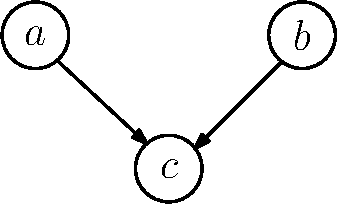
\includegraphics[height = 2cm]{./figures/bayesnet}
\hfill
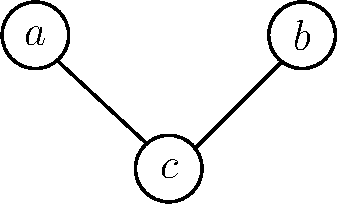
\includegraphics[height = 2cm]{./figures/mrf}
\hfill
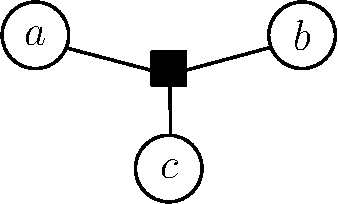
\includegraphics[height = 2cm]{./figures/factor_graph}
\end{figure}

Three types of probabilistic graphical models:
\begin{itemize}
\item \cemph{Bayesian networks (directed graphical models)}
\item \cemph{Markov random fields (undirected graphical models)}
\item \cemph{Factor graphs}
\end{itemize}
\pause
\begin{itemize}
\item \textbf{Nodes:} (Sets of) random variables
\item \textbf{Edges:} Probabilistic/functional relations between variables
\end{itemize}

\pause
\arrow Graph captures the \cemph{way in which the joint distribution over all
random variables can be decomposed} into a product of factors depending
only on a subset of these variables

\end{frame}



%%%%%%%%%%%%%%%%%%%%%%%%%%%%%%%%%%%%%%%%%%%%%%%%%%%%%%

% \begin{frame}
% \frametitle{Why are they useful?}
% \begin{itemize}[<+->]
% \item Simple way to \cemph{visualize the structure} of a probabilistic
%   model
% \item \cemph{Insights into properties} of the model (e.g., conditional
%   independence) by inspection of the graph
% \item Can be used to \cemph{design/motivate new models}
% \item Complex computations for inference and learning can be expressed
%   in terms of \cemph{graphical manipulations} 
% \end{itemize}
% \end{frame}

%%%%%%%%%%%%%%%%%%%%%%%%%%%%%%%%%%%%%%%%%%%%%%%%%%%%%%
\begin{frame}
\frametitle{Importance of Visualization}
\vspace{-5mm}
\begin{figure}
\centering
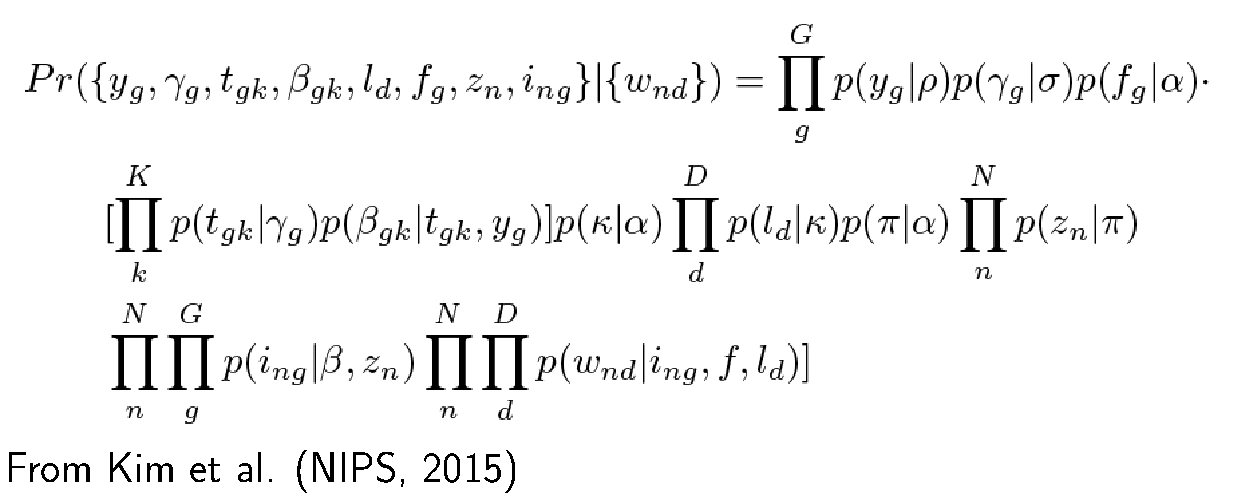
\includegraphics[width = 0.7\hsize]{./figures/ex1b}\\
\pause
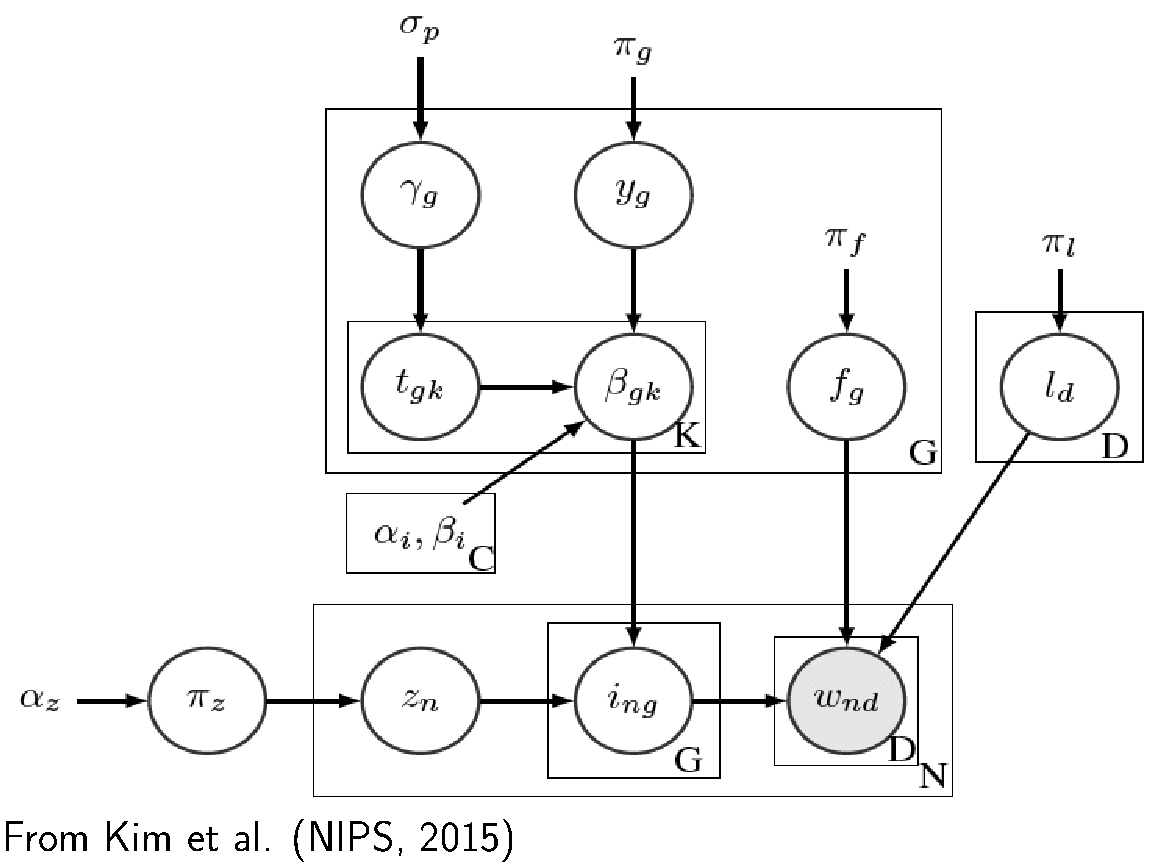
\includegraphics[height = 4.7cm]{./figures/ex1}\nocite{Kim2015}
\end{figure}


\end{frame}

%%%%%%%%%%%%%%%%%%%%%%%%%%%%%%%%%%%%%%%%%%%%%%%%%%%%%%
\begin{frame}
\frametitle{}
\begin{center}
{\Large \emph{Expressing Factorisations as Graphs}} \\

\end{center}
\end{frame}


%%%%%%%%%%%%%%%%%%%%%%%%%%%%%%%%%%%%%%%%%%%%%%%%%%%%%%
\begin{frame}{Directed Graphical Models}
  \begin{figure}
    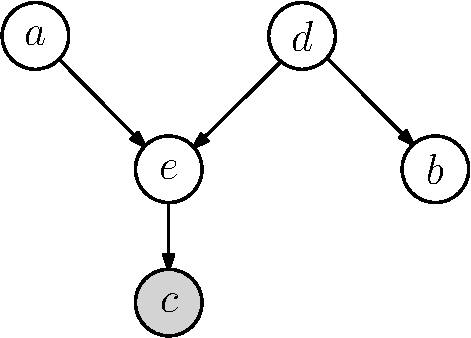
\includegraphics[height = 4cm]{./figures/d-separation1}
  \end{figure}
  \begin{itemize}
  \item Nodes: Random variables
  \item Shaded nodes: Observed random variables
  \item Unshaded nodes: Unobserved (latent) random variables
    \item Directed arrow from $a$ to $b$: Conditional distribution
      $p(b|a)$. 
  \end{itemize}
  
\end{frame}
%%%%%%%%%%%%%%%%%%%%%%%%%%%%%%%%%%%%%%%%%%%%%%%%%%%%%% 

\begin{frame}
\frametitle{Skill: From Joints to Graphs}
Consider the joint distribution
\begin{align*}
p(a,b,c) = p(c|a,b)p(b|a)p(a)
\end{align*}

Building the corresponding graphical model:
\begin{enumerate}[<+->]
\item Create a node for all random variables
\item For each conditional distribution, we add a directed link (arrow) to
the graph from the nodes corresponding to the variables on which the
distribution is conditioned on
\end{enumerate}

\begin{figure}
\centering
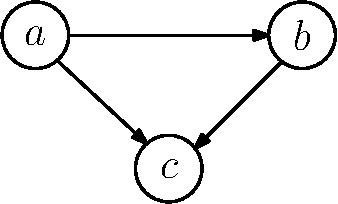
\includegraphics[height = 2cm]{./figures/bayesnet2}
\end{figure}
\onslide+<3->{
\arrow Graph layout depends on the choice of factorization
}
\end{frame}



% %%%%%%%%%%%%%%%%%%%%%%%%%%


\begin{frame}
\frametitle{Skill: From Graphs to Joints}
\begin{figure}
\centering
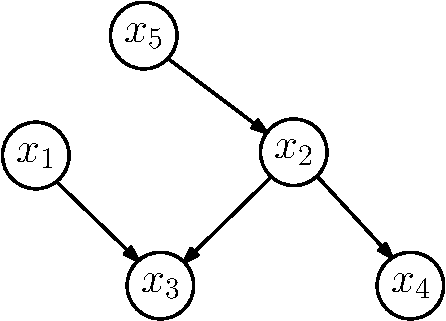
\includegraphics[height=3cm]{./figures/bayesnet3}
\end{figure}
\begin{itemize}
\item \cemph{Joint distribution is the product of a set of conditionals}, one
  for each node in the graph
  \pause
\item Each conditional depends only on the \cemph{parents of the
corresponding node} in the graph
\end{itemize}
\pause
\vspace{-2mm}
\begin{align*}
p(x_1,x_2,x_3,x_4,x_5) = p(x_1)p(x_5)p(x_2|x_5)p(x_3|x_1,x_2)p(x_4|x_2)
\end{align*}
\pause
In general:\qquad
$
\colchar{$p(\vec x) = p(x_1, \dotsc, x_K) = \prod_{k = 1}^Kp(x_k|\text{parents}(x_k))$}{blue}
$

\end{frame}


\begin{frame}{What is \emph{the} graphical model?}
Remember, a model is defined simply by its joint distribution, which often is just between data and a latent variable:
\begin{align}
p(\vx, \vz)
\end{align} \pause
We can factorise this in two distinct, but equally valid ways:
\begin{align}
p(\vx, \vz) = p(\vx|\vz)p(\vz) = p(\vx) p(\vz|\vx)
\end{align}\pause
\vspace{-0.3cm}
\begin{columns}
\column{0.5\hsize}
\centering
      \tikz{ %
        \node[latent] (x) {$\vx$} ; %
        \node[latent, left=of x] (z) {$\vz$} ; %
        \edge {x} {z} ; %
      }
\column{0.5\hsize}
\centering
      \tikz{ %
        \node[latent] (x) {$\vx$} ; %
        \node[latent, left=of x] (z) {$\vz$} ; %
        \edge {z} {x} ; %
      }
\end{columns}
\vspace{0.3cm}

Which one is correct? \pause Depends on which conditional you specified!
\begin{align}
p(\vx, \vz) = \colchar{$p(\vx|\vz)$}{green}\colchar{$p(\vz)$}{green} = \colchar{$p(\vx)$}{red} \colchar{$p(\vz|\vx)$}{red}
\end{align}
\end{frame}



%%%%%%%%%%%%%%%%%%%%%%%%%%%%%%%%%%%%%%%%%%%%%%%%%%%%%%

\begin{frame}
\frametitle{Graphical Model for (Bayesian) Linear Regression}

\begin{columns}
\column{0.5\hsize}
\begin{figure}
\centering
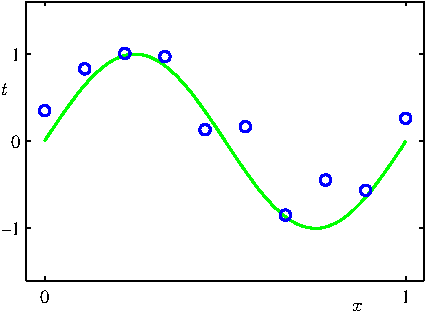
\includegraphics[width = \hsize]{./figures/Figure1_2}\\
\tiny{From PRML (Bishop, 2006)\nocite{Bishop2006}}
\end{figure}
\column{0.5\hsize}
We are given a data set $(x_1,y_1), \dotsc, (x_N,y_N)$ where
\begin{align*}
y_i = f(x_i) + \varepsilon, \quad \varepsilon\sim\gauss{0}{\sigma^2}
\end{align*}
with $f$ unknown. \\
\arrow Find a (regression) model that explains the data
\end{columns}

\pause
\begin{itemize}
\item Consider \cemph{polynomials}
$
f(x) = \sum_{j=0}^M w_j x^j
$
with parameters $\vec w = [w_0,\dotsc,w_M]\T$. 
\item \cemph{Bayesian linear regression:} Place a conjugate Gaussian prior on
  the parameters: $p(\vec w) = \gauss{\vec 0}{\alpha^2\mat I}$
\end{itemize}


\end{frame}


%%%%%%%%%%%%%%%%%%%%%%%%%%%%%%%%%%%%%%%%%%%%%%%%%%%%%%

\begin{frame}[t]
\frametitle{Graphical Model for Linear Regression}

\begin{columns}
\column{0.35\hsize}
\begin{figure}
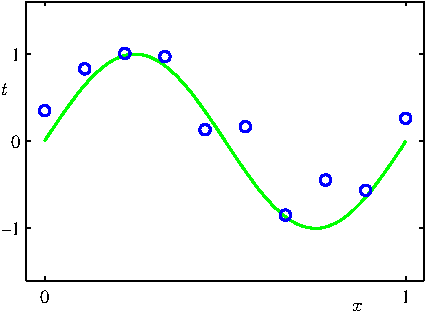
\includegraphics[width =\hsize]{./figures/Figure1_2}\\
\tiny{From PRML (Bishop, 2006)}
\end{figure}
\column{0.5\hsize}
\begin{align*}
p(y_i|\vec w,x_i) &= \gaussx{y_i}{f_{\vec w}(x_i)}{\sigma^2}\\
%\varepsilon &\sim\gauss{0}{\sigma^2}\\
f(x) &=\sum_{j=0}^M w_j x^j\\
p(\vec w) &=\gauss{\vec 0}{ \alpha^2\mat I}
\end{align*}
\end{columns} \pause
\begin{figure}
\centering
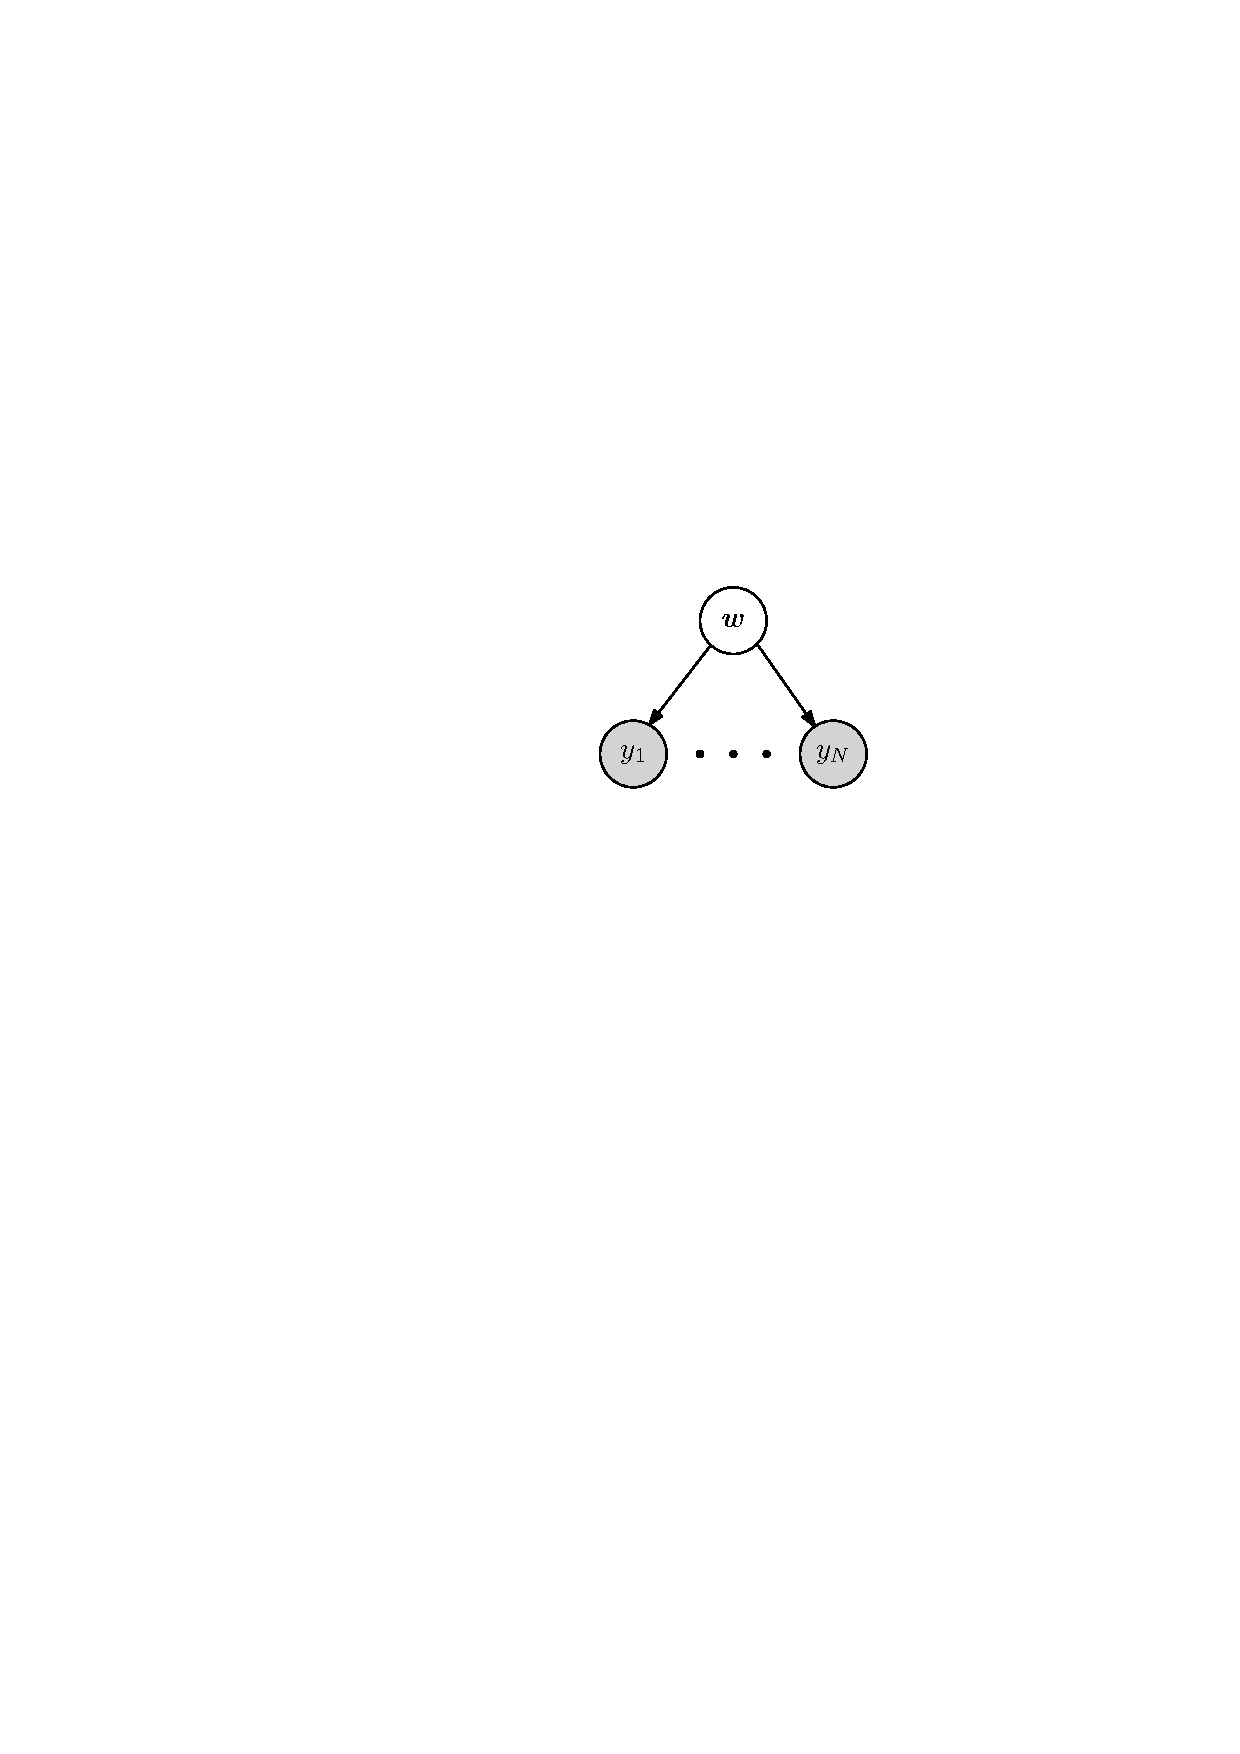
\includegraphics[height = 3cm]{./figures/gm_bayesian_regression1}
\hfill
\pause
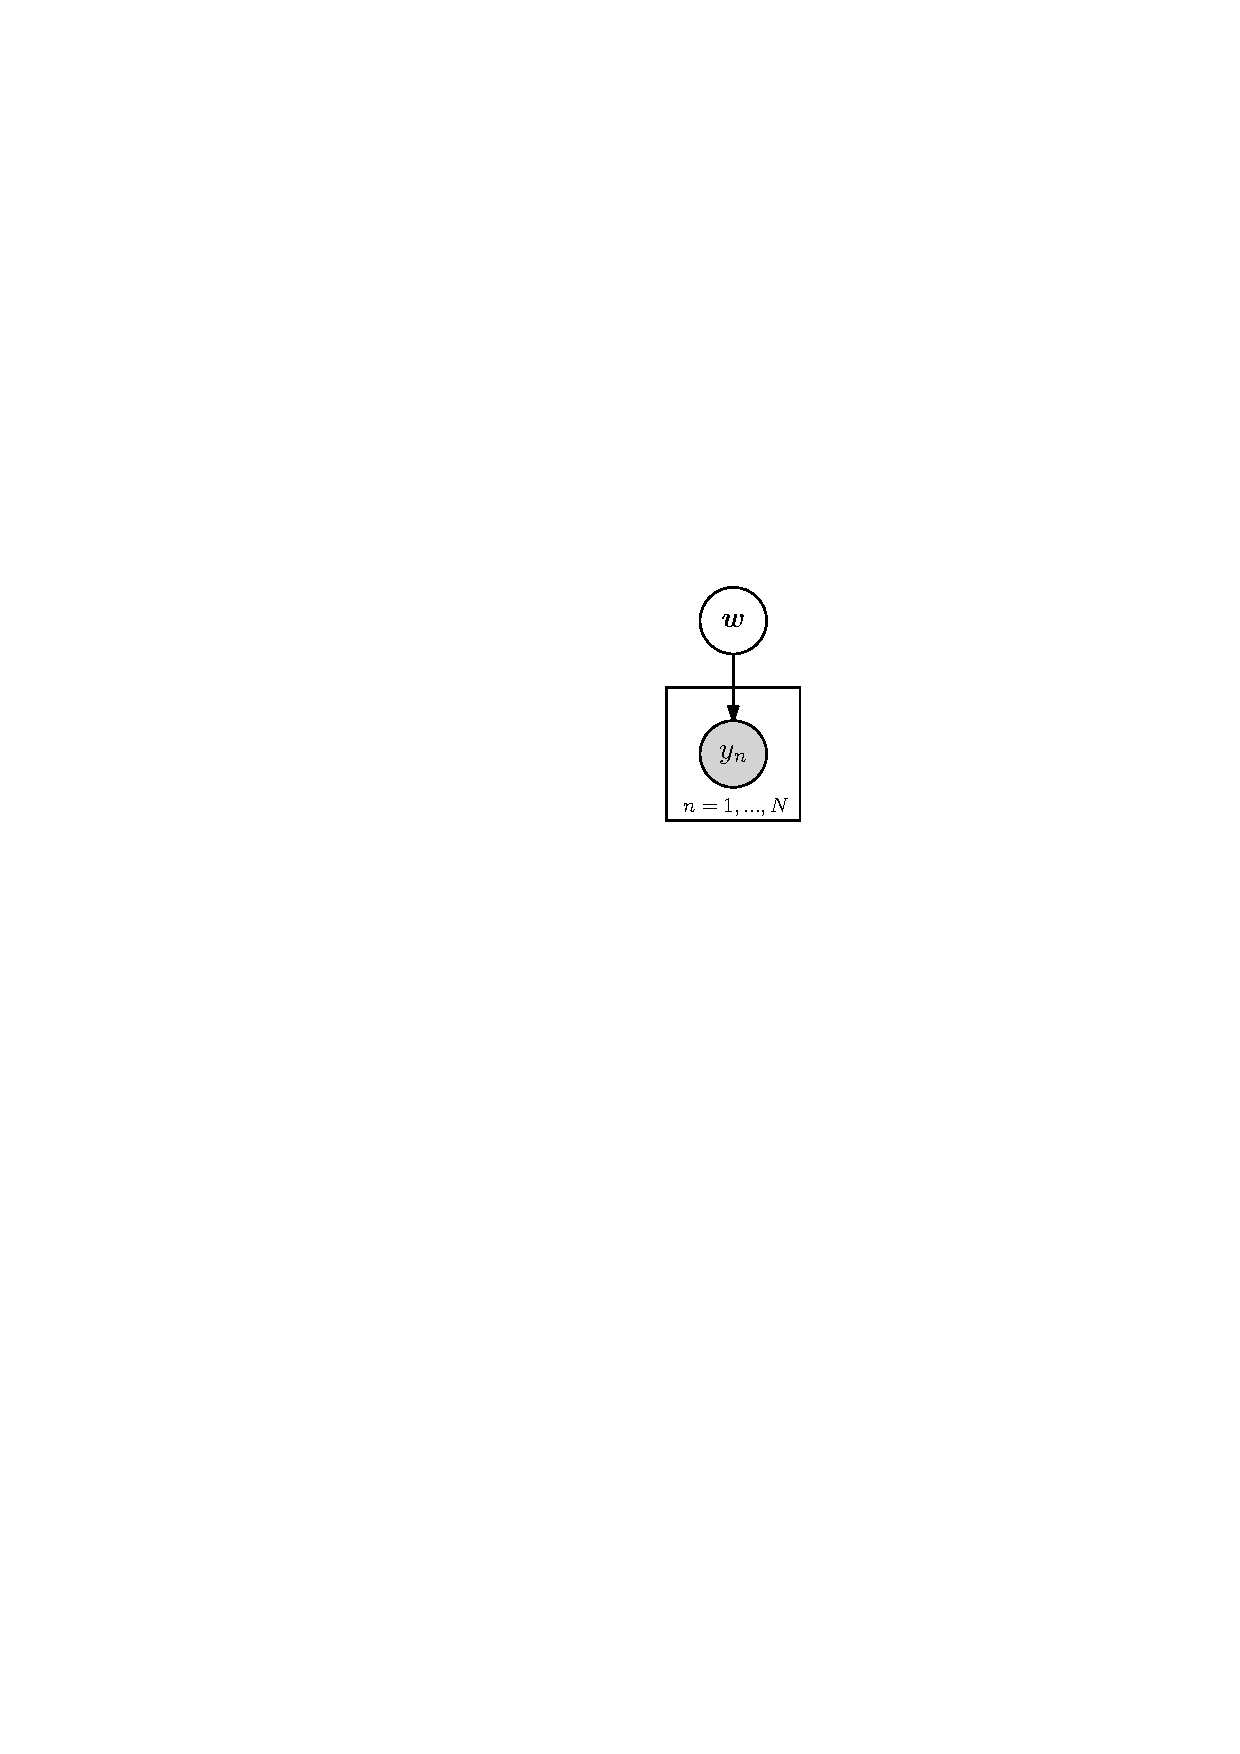
\includegraphics[height =
3cm]{./figures/gm_plate_bayesian_regression1}
\hfill
\pause
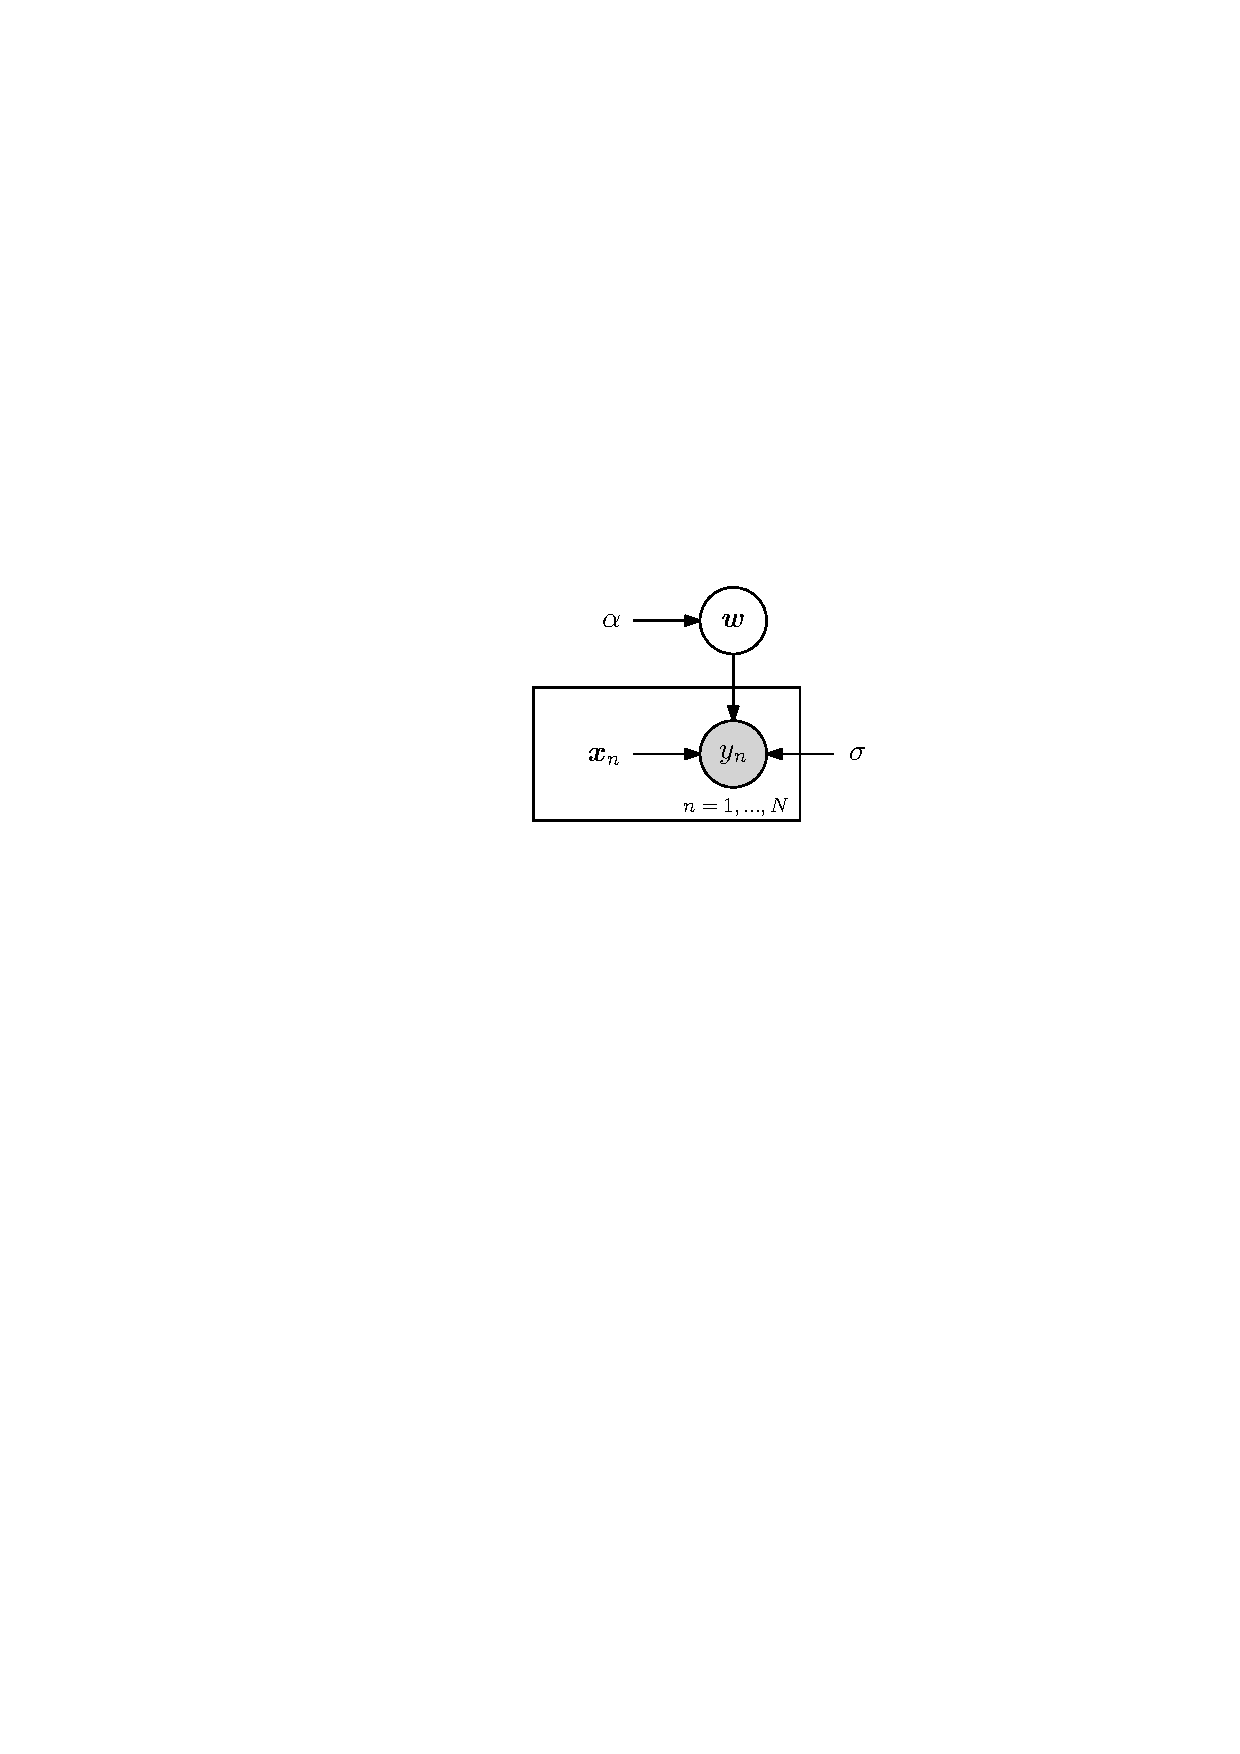
\includegraphics[height = 3cm]{./figures/gm_plate_bayesian_regression2}
\end{figure}


\end{frame}

%%%%%%%%%%%%%%%%%%%%%%%%%%%%%%%%%%%%%%%%%%%%%%%%%%%%%%


\begin{frame}
\frametitle{}
\begin{center}
{\Large \emph{Finding Conditional Independence}} \\
\end{center}
\end{frame}




\begin{frame}
\frametitle{Conditional Independence}
% \begin{figure}
% \centering
% 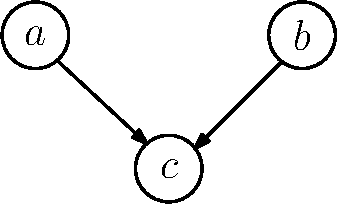
\includegraphics[height = 2cm]{./figures/bayesnet}
% \end{figure}
\begin{center}
      \tikz{ %
        \node[latent] (a) {$a$} ; %
        \node[latent, right=of a] (b) {$b$} ; %
        \node[latent, above=of a] (c) {$c$} ;
%        \node[latent, left=of x] (z) {$\vz$} ; %
        \edge {c} {a} ; %
        \edge {c} {b} ; %
      }
\end{center}
\begin{align*}
  a \ci b | c &\iff p(a,b|c) = p(a|c)p(b|c) \\
  &\iff p(a|b,c) = p(a|c)
\end{align*}

\vspace{-0.3cm}

\begin{itemize}
\item (Conditional) independence allows for a \cemph{factorization of the
  joint distribution} \arrow More efficient inference
\begin{align}
\Exp{p(a,b|c)}{f(a)g(b)} = \Exp{p(a|c)}{f(a)}\cdot\Exp{p(b|c)}{g(b)}
\end{align}
\item \cemph{Conditional independence} properties of the joint
  distribution can be read directly from the graph without analytical manipulations!
\end{itemize}
\arrow \emph{d-separation} (Pearl, 1988\nocite{Pearl1988})

\end{frame}
%%%%%%%%%%%%%%%%%%%%%%%%%%%%%%%%%%%%%%%%%%%%%%%%%%%%%%

\begin{frame}
\frametitle{D-Separation (Directed Graphs)}

\begin{columns}
\column{0.4\hsize}
\begin{figure}
\centering
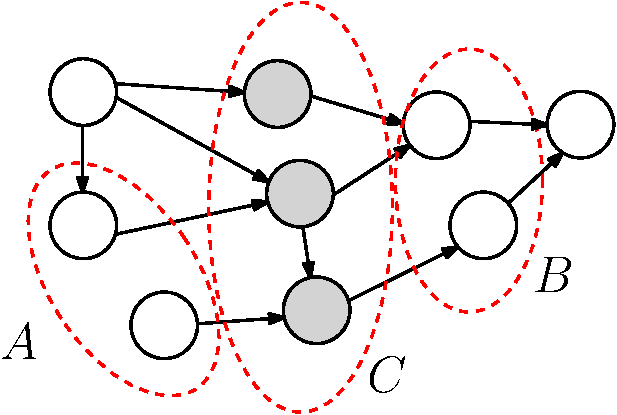
\includegraphics[height = 3cm]{./figures/d-separation}
\end{figure}
\column{0.6\hsize} Directed, acyclic graph in which $A,B,C$ are
arbitrary, non-intersecting sets of nodes. Does $A\ci B|C$
hold?\newline Note: $C$ is observed if we condition on it (and the
nodes in the GM are shaded)
\end{columns}
\pause
\vspace{0.5mm}
\arrow Consider \cemph{all possible paths} from any node in $A$ to any node in
$B$.
\pause
\newline Any such \emph{path is blocked} if it includes a node
such that either
\begin{itemize}
\item Arrows on the path meet either \cemph{head-to-tail or
    tail-to-tail} at the node, \underline{and} the node is in the set
  $C$ or
  \pause
\item Arrows meet \cemph{head-to-head} at the node \underline{and}
  neither the node nor any of its descendants is in the set $C$
\end{itemize}
\pause
If \cemph{all paths are blocked}, then $A$ is \cemph{d-separated}
(conditionally indep.) from
$B$ by $C$, and the joint distribution satisfies $A\ci B|C$.


\end{frame}

%%%%%%%%%%%%%%%%%%%%%%%%%%%%%%%%%%%%%%%%%%%%%%%%%%%%%%
\begin{frame}
\frametitle{Exam skill: Find conditional independencies}
\begin{figure}
\centering
\subfloat[$a\ci b|c$?]{
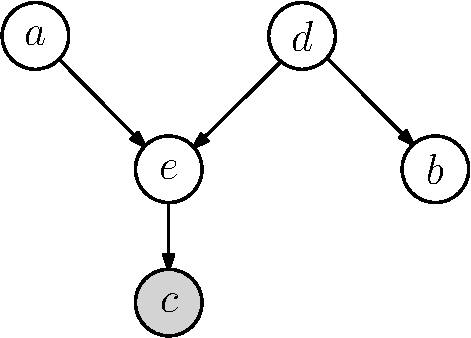
\includegraphics[height = 3cm]{./figures/d-separation1}
% unblocked (arrows meet head-to-head in e, and c (descendant of e) is observed
}
\hspace{1cm}
\subfloat[$a\ci b|d$?]{
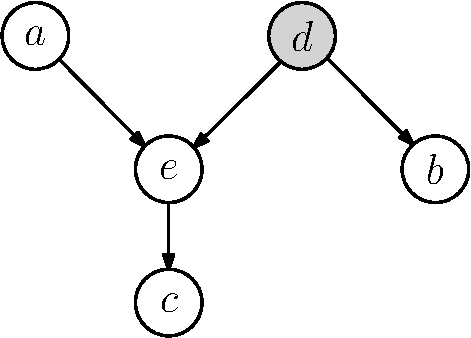
\includegraphics[height = 3cm]{./figures/d-separation2}
% blocked for 2 reasons:
% (1) d has tail-to-tail arrows and is observed
% (2) e has head-to-head arrows and neither e nor its descendants are observed
}
\end{figure}
\begin{myblock}{}
A path is \emph{blocked} if it includes a node such that either
\begin{itemize}
\item The arrows on the path meet either head-to-tail or tail-to-tail at the
node, and the node is in the set $C$ (observed) or
\item The arrows meet head-to-head at the node, and neither the node nor any
of its descendants is in the set $C$ (observed) 
\end{itemize}
\end{myblock}
\end{frame}




\begin{frame}{Markov Chains}
\begin{center}
\scalebox{0.7}{
      \tikz{ %
        \node[latent] (x1) {$x_1$} ; %
        \node[latent, right=of x1] (x2) {$x_2$} ; %
        \node[latent, right=of x2] (x3) {$x_3$} ; %
        \node[latent, right=of x3] (x4) {$x_4$} ; %
        \node[latent, right=of x4] (x5) {$x_5$} ; %
        \node[obs, below=of x1] (y1) {$y_1$} ; %
        \node[obs, below=of x2] (y2) {$y_2$} ; %
        \node[obs, below=of x3] (y3) {$y_3$} ; %
        \node[obs, below=of x4] (y4) {$y_4$} ; %
        \node[latent, below=of x5] (y5) {$y_5$} ; %
        \edge {x1} {x2} ; %
        \edge {x2} {x3} ; %
        \edge {x3} {x4} ; %
        \edge {x4} {x5} ; %
        \edge {x1} {y1} ; %
        \edge {x2} {y2} ; %
        \edge {x3} {y3} ; %
        \edge {x4} {y4} ; %
        \edge {x5} {y5} ; %
      }
}
\end{center}
\vspace{-0.2cm}
\begin{align}
p(\{x_t\}_{t=1}^5, \{y_t\}_{t=1}^5) = p(x_1) \left[\prod_{t=2}^5 p(x_t|x_{t-1})\right] \left[\prod_{t=1}^5 p(y_t|x_t)\right]
\end{align}
How do we compute the posterior on $x_5$ (so we can predict $y_5$)? \pause
\begin{itemize}
\item We note that $x_4 \ci \{x_t\}_{t=1}^2, \{y_t\}_{t=1}^3 | x_3$  (blocked path, tail-to-tail) \\
  $p(x_4|\{y_t\}_{t=1}^4) = \int p(x_4|x_3, y_4) p(x_3|\{y_t\}_{t=1}^3) \calcd x_3$ \pause
\item This can be applied recursively!\pause
\item Finding the posterior can be done in linear time!
\end{itemize}
\end{frame}


\begin{frame}{Recommended Reading}
  \begin{center}
    Bishop: Pattern Recognition and Machine Learning, Chapter 8 \\
    Directed graphical models
  \end{center}
\end{frame}





%%%%%%%%%%%%%%%%%%%%%%%%%%%%%%%%%%%%%%%%%
% REFERENCES
%%%%%%%%%%%%%%%%%%%%%%%%%%%%%%%%%%%%%%%%%
\begin{frame}[t,allowframebreaks]
\frametitle{References}
\linespread{1.0}
\tiny
\bibliographystyle{abbrv}
\bibliography{../references.bib}
\end{frame}




\begin{frame}
\frametitle{}
\begin{center}
{\Large \emph{Not examinable from here}} \\
\end{center}
\end{frame}



\begin{frame}
\frametitle{}

\begin{center}
{\Large \emph{Factor Graphs}} \\
A different graphical representation
\end{center}
Good references:\\[3mm]
Kschischang et al.: Factor Graphs and the Sum-Product Algorithm. IEEE
Transactions on Information Theory (2001)\\[2mm]
Loeliger: An Introduction to Factor Graphs. IEEE Signal Processing
Magazine, (2004)\nocite{Kschischang2001,Loeliger2004}
\end{frame}



%%%%%%%%%%%%%%%%%%%%%%%%%%%%%%%%%%%%%%%%%%%%%%%%%%%%%%
\begin{frame}
\frametitle{Factor Graphs}

\begin{figure}
\centering
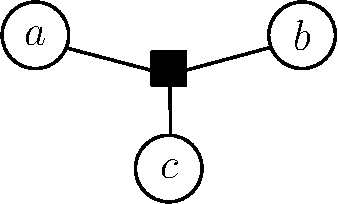
\includegraphics[height = 3cm]{./figures/factor_graph}
\end{figure}

\begin{itemize}
\item (Un)directed graphical models express a global function of
  several variables as a product of factors over subsets of those
  variables
\item Factor graphs make this decomposition explicit by introducing
  \cemph{additional nodes for the factors} themselves

\end{itemize}

\end{frame}

%%%%%%%%%%%%%%%%%%%%%%%%%%%%%%%%%%%%%%%%%%%%%%%%%%%%%%
\begin{frame}
\frametitle{Factorizing the Joint}
The joint distribution is a product of factors:
\begin{align*}
p(\vec x) = \prod_s f_s(\vec x_s)
\end{align*}

\begin{itemize}
\item $\vec x = (x_1,\dotsc, x_n)$
\item $\vec x_s$: Subset of variables
\item $f_s$: Factor; non-negative function of the variables $\vec x_s$
\end{itemize}

\pause
\begin{itemize}
\item Building a factor graph as a \cemph{bipartite graph:}
\begin{itemize}
\item Nodes for all random variables (same as in (un)directed
  graphical models)
\item Additional nodes for factors (black squares) in the joint
  distribution
\end{itemize}
\item Undirected links connecting each factor node to all of the
  variable nodes the factor depends on
\end{itemize}


\end{frame}

%%%%%%%%%%%%%%%%%%%%%%%%%%%%%%%%%%%%%%%%%%%%%%%%%%%%%%
\begin{frame}
\frametitle{Example}

\begin{figure}
\centering
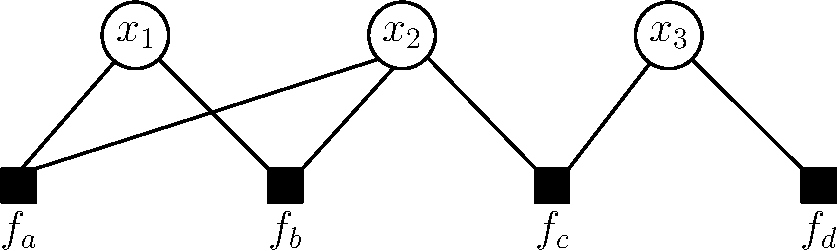
\includegraphics[height = 3cm]{./figures/fac_graph_ex1}
\end{figure}

\begin{align*}
p(\vec x) = f_a(x_1, x_2)f_b(x_1,x_2)f_c(x_2,x_3)f_d(x_3)
\end{align*}

\pause
\arrow Efficient inference algorithms for factor graphs (e.g.,
\cemph{sum-product algorithm})
\end{frame}









%%%%%%%%%%%%%%%%%%%%%%%%%%%%%%%%%%%%%%%%%%%%%%%%%%%%%%

\begin{frame}
\frametitle{Directed Graphical Model $\to$ Factor Graph}

\begin{enumerate}
\item Take variable nodes from Bayesian network
\item Create additional factor nodes corresponding to the conditional distributions
\item Add appropriate links
\end{enumerate}

Not unique



\end{frame}

%%%%%%%%%%%%%%%%%%%%%%%%%%%%%%%%%%%%%%%%%%%%%%%%%%%%%%
\begin{frame}
\frametitle{Example: Directed Graph $\to$ Factor Graph}

\begin{figure}
\centering
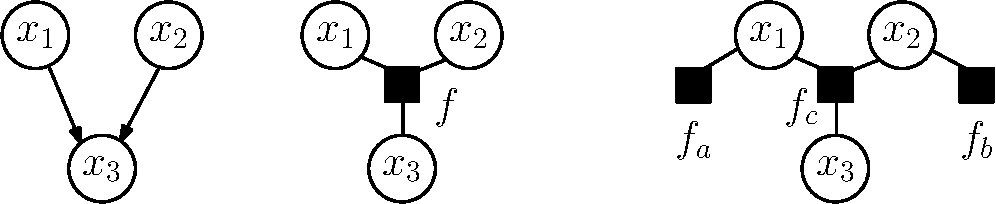
\includegraphics[width = \hsize]{./figures/dgm2fac}
\end{figure}

\begin{itemize}
\item Directed graph with factorization $p(x_1)p(x_2)p(x_3|x_1,x_2)$
\item Factor graph with factor $f(x_1,x_2,x_3) = p(x_1)p(x_2)p(x_3|x_1,x_2)$
\item Factor graph with factors $f_a=p(x_1),~f_b = p(x_2),~f_c = p(x_3|x_1,x_2)$
\end{itemize}



\end{frame}

%%%%%%%%%%%%%%%%%%%%%%%%%%%%%%%%%%%%%%%%%%%%%%%%%%%%%%
\begin{frame}
\frametitle{Removing Cycles}

\begin{figure}
\centering
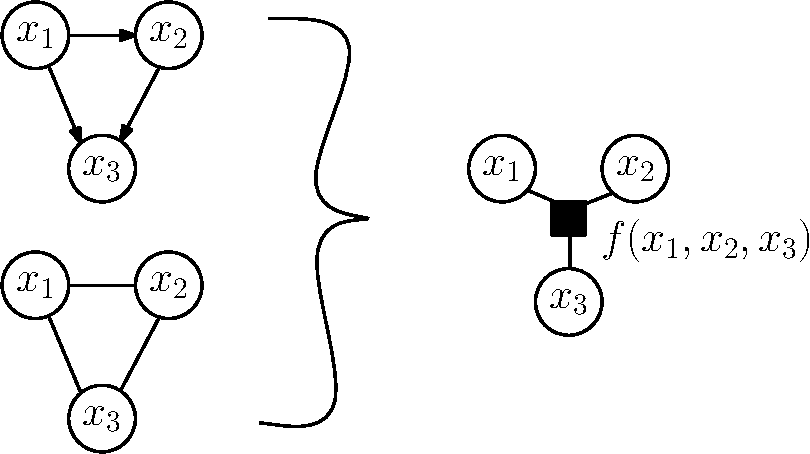
\includegraphics[width = 0.22\hsize,trim=0 4.2cm 10cm 0,clip]{./figures/remove_loops}
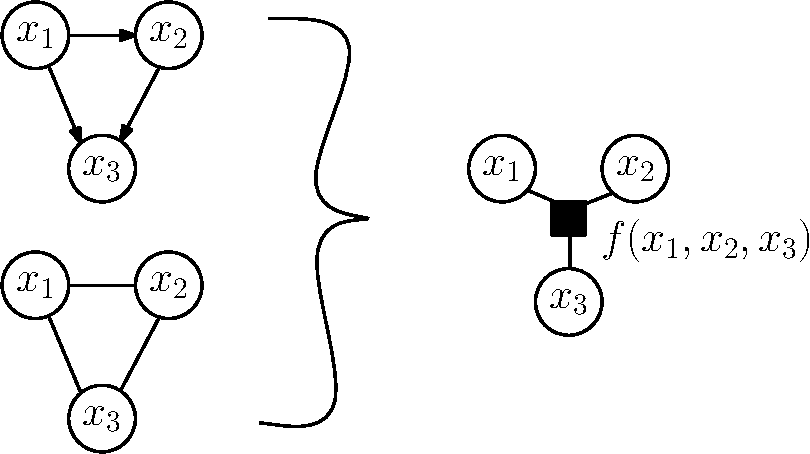
\includegraphics[width = 0.4\hsize,trim=7cm 2cm 0cm 2cm,clip]{./figures/remove_loops}
\end{figure}
\begin{equation}
p(x_3|x_2, x_1)p(x_2|x_1)p(x_1) = f_a(x_1, x_2, x_3)f_b(x_1, x_2)f_c(x_2) = f(x_1, x_2, x_3)
\end{equation}

\begin{itemize}
\item Local cycles in an (un)directed graph (due to links connecting
  parents of a node) can be removed on conversion to a factor graph
\end{itemize}

\end{frame}

%%%%%%%%%%%%%%%%%%%%%%%%%%%%%%%%%%%%%%%%%%%%%%%%%%%%%%
\begin{frame}
\frametitle{}

\begin{center}
{\Large \emph{Exact Inference in Factor Graphs}}

\end{center}
\end{frame}
%%%%%%%%%%%%%%%%%%%%%%%%%%%%%%%%%%%%%%%%%%%%%%%%%%%%%% 

\begin{frame}
\frametitle{Sum-Product Algorithm for Factor Graphs}

\begin{itemize}
\item Factor graphs give a \cemph{uniform treatment to message
    passing}, which is used for inference in graphs
\item Inference: Find (marginal) posterior distributions
  \pause
\item Idea: \cemph{Local message passing} between nodes and factors
\item Two different types of messages: 
\begin{itemize}
\item Messages $\mu_{x\to f}(x)$ from variable nodes to factors
\item Messages $\mu_{f\to x}(x)$ from factors to variable nodes
\end{itemize}
\pause
\item Repeated sending of these messages through the graph converges
\item Factors transform messages into evidence for the receiving node
\end{itemize}

\end{frame}


% %%%%%%%%%%%%%%%%%%%%%%%%%%%%%%%%%%%%%%%%%%%%%%%%%%%%%%

% \begin{frame}
% \frametitle{Problem 1: Find a Marginal}

% \begin{itemize}
%   \item 
%  Assume all variables are hidden (for the time being)
% \item 
% By definition (sum rule): 
% \begin{align*}
% p(x) = \sum_{\vec x\backslash x}p(\vec x)
% \end{align*}
% \end{itemize}
% \end{frame}


%%%%%%%%%%%%%%%%%%%%%%%%%%%%%%%%%%%%%%%%%%%%%%%%%%%%%%

\begin{frame}
\frametitle{Variable-to-Factor Message}

\begin{figure}
\centering
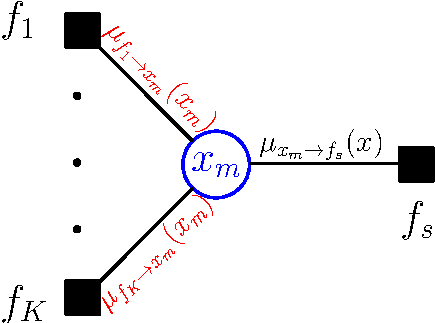
\includegraphics[height=3.5cm]{./figures/var2fac_msg}
\end{figure}
\vspace{-5mm}
\begin{align*}
\mu_{x_m\to f_s}(x_m) = \prod_{l\in\text{ne}(x_m)\backslash f_s}
\red{\mu_{f_l\to x_m}(x_m)}
\end{align*}

\begin{itemize}[<+->]
\item Take the product of all \red{incoming messages along all other links}
\item A variable node can send a message to a factor node once it has
  received messages from all other neighboring factors
\item The message that a node sends to a factor is made up of the
  messages that it receives from all other factors.
\end{itemize}

\end{frame}



%%%%%%%%%%%%%%%%%%%%%%%%%%%%%%%%%%%%%%%%%%%%%%%%%%%%%%

\begin{frame}
  \frametitle{Factor-to-Variable Message}
\begin{figure}
\centering
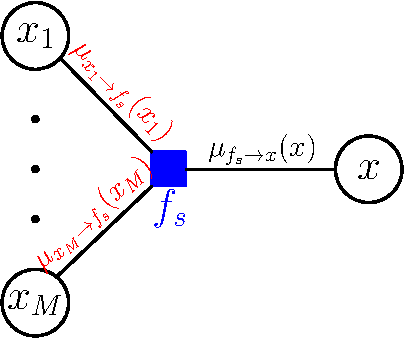
\includegraphics[height=3cm]{./figures/fac2var_msg}
\end{figure}
\vspace{-5mm}

\begin{align*}
\mu_{f_s\to x}(x) = \onslide+<3->{\orange{\sum_{x_1}\cdots\sum_{x_M}}}\onslide+<2->{\blue{f_s(x, x_1,\dotsc, x_M)}}\red{\prod_{m\in\text{ne}(f_s)\backslash x}\mu_{x_m\to f_s}(x_m)}
\end{align*}

\begin{itemize}[<+->]
\item \red{Take the product of the incoming messages along all other links
  coming into the factor node}
\item \blue{Multiply by the factor associated with that node}
\item \orange{Marginalize over all variables associated with the
  \underline{incoming} messages}

\end{itemize}

\end{frame}


%%%%%%%%%%%%%%%%%%%%%%%%%%%%%%%%%%%%%%%%%%%%%%%%%%%%%%

\begin{frame}
\frametitle{Initialization}

\begin{itemize}
\item 
If the leaf node is a \cemph{variable node}, initialize the corresponding messages
to 1:
\begin{align*}
\mu_{x\to f}(x) = 1
\end{align*}
\item If the leaf node is a \cemph{factor node}, the message should be
\begin{align*}
\mu_{f\to x}(x) = f(x)
\end{align*}
\end{itemize}
\end{frame}



%%%%%%%%%%%%%%%%%%%%%%%%%%%%%%%%%%%%%%%%%%%%%%%%%%%%%%
\begin{frame}
\frametitle{Example (1)}

\begin{columns}
\column{0.5\hsize}
\begin{figure}
\centering
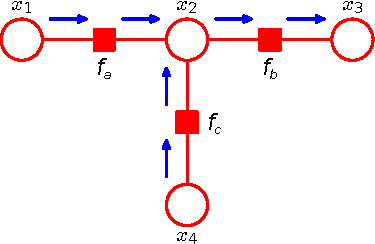
\includegraphics[height = 3cm]{./figures/Figure8_52a}\\
\tiny{From PRML (Bishop, 2006)}
\end{figure}
\column{0.5\hsize}
\begin{align*}
  \mu_{x_1\to f_a}(x_1) &= 1\\
\mu_{f_a\to x_2}(x_2) &= \sum_{x_1} f_a(x_1,x_2)\cdot 1\\
\mu_{x_4\to f_c}(x_4) &= 1\\
\mu_{f_c\to x_2}(x_2)  &= \sum_{x_4} f_c(x_2,x_4)\cdot 1\\
\mu_{x_2\to f_b}(x_2) &= \mu_{f_a\to x_2} (x_2)\mu_{f_c\to x_2} (x_2)\\
\mu_{f_b\to x_3}(x_3) &= \sum_{x_2}f_b(x_2, x_3) \mu_{x_2\to f_b}(x_2)
\end{align*}
\end{columns}
\end{frame}


%%%%%%%%%%%%%%%%%%%%%%%%%%%%%%%%%%%%%%%%%%%%%%%%%%%%%%
\begin{frame}
\frametitle{Example (2)}

\begin{columns}
\column{0.5\hsize}
\begin{figure}
\centering
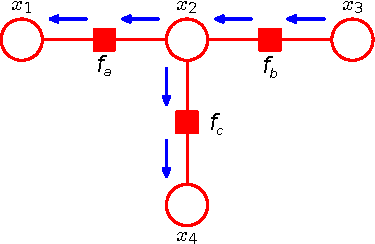
\includegraphics[height = 3cm]{./figures/Figure8_52b}\\
\tiny{From PRML (Bishop, 2006)}
\end{figure}
\column{0.5\hsize}
\begin{align*}
\mu_{x_3\to f_b}(x_3) &= 1
\\
\mu_{f_b\to x_2}(x_2) &= \sum_{x_3} f_b(x_2,x_3)\cdot 1
\\
\mu_{x_2\to f_a}(x_2) &= \mu_{f_b\to x_2}(x_2)\mu_{f_c\to x_2}(x_2)
\\
\mu_{f_a\to x_1}(x_1)  &= \sum_{x_2} f_a(x_1,x_2)\mu_{x_2\to f_a}(x_2)
\\
\mu_{x_2\to f_c}(x_2) &= \mu_{f_a\to x_2} (x_2)\mu_{f_b\to x_2} (x_2)
\\
\mu_{f_c\to x_4}(x_4) &= \sum_{x_2}f_c(x_2, x_4) \mu_{x_2\to f_c}(x_2)
\end{align*}
\end{columns}

\end{frame}

%%%%%%%%%%%%%%%%%%%%%%%%%%%%%%%%%%%%%%%%%%%%%%%%%%%%%%

\begin{frame}
\frametitle{Marginals}

\begin{figure}
\centering
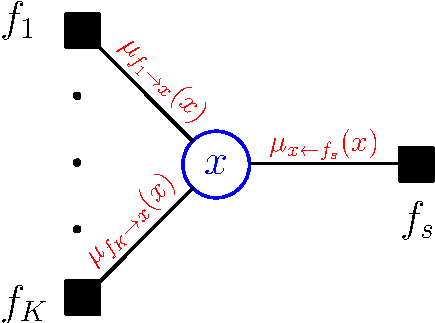
\includegraphics[height = 5cm]{./figures/marginal_computation_fac}
\end{figure}

For a single variable node the marginal is given as the \cemph{product of all
incoming messages:}
\begin{align*}
\blue{p(x)} = \prod_{f_i\in\text{ne}(x)} \red{\mu_{f_i\to x}(x)}
\end{align*}

\end{frame}


%%%%%%%%%%%%%%%%%%%%%%%%%%%%%%%%%%%%%%%%%%%%%%%%%%%%%%

\begin{frame}
\frametitle{Observed Variables \arrow Posterior}

\begin{itemize}
\item Thus far, we have focused on the case where all variables are
unobserved.
\item Posterior is always conditioned on observations
\item Partition $\vec x = \vec h \cup \vec v$, $\vec h$: hidden variables, $\vec
  v$: visible variables with observations $\hat {\vec v}$
\item $p(\vec v = \hat{\vec v}) = \prod_{i} I(v_i = \hat v_i)$
\item $p(\vec x) p(\vec v = \hat{\vec v}) = p(\vec h, \vec v =
  \hat{\vec v}) ~\propto~ p(\vec h|\vec v = \hat{\vec v})$
\item \cemph{Marginal posteriors} $p(h_i|\vec v = \hat{\vec v})$ can
  be obtained via sum-product algorithm and some local computations\\
  \arrow (Koller \& Friedman, 2009)\nocite{Koller2009}
 \end{itemize}

\end{frame}

%%%%%%%%%%%%%%%%%%%%%%%%%%%%%%%%%%%%%%%%%%%%%%%%%%%%%%
\begin{frame}{Exact Inference in (Un)Directed Graphical Models}

  \begin{itemize}
  \item Loops are possible \arrow \emph{Junction Tree Algorithm}
    (Lauritzen \& Spiegelhalter, 1988)\nocite{Lauritzen1988}
  \item Alternative: \emph{Loopy Belief Propagation} (Frey \& MacKay
    1998)\nocite{Frey1998}
  \end{itemize}
  
\end{frame}


%%%%%%%%%%%%%%%%%%%%%%%%%%%%%%%%%%%%%%%%%%%%%%%%%%%%%%
\begin{frame}
  \frametitle{Applications of Inference in Graphical Models}
\begin{figure}
\centering

\includegraphics[height = 2.5cm]{./figures/trueskill_example}
\hfill
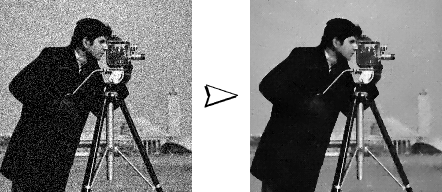
\includegraphics[height = 2.5cm]{./figures/image_denoising_example}
\end{figure}

\begin{itemize}
\item \cemph{Ranking:} TrueSkill {\small (Herbrich et al., 2007)\nocite{Herbrich2007}}
\item \cemph{Computer vision:} de-noising, segmentation, semantic
  labeling, ... {\small{(e.g., Sucar \& Gillies, 1994; Shotton et al.,
    2006; Szeliski et al., 2008) }\nocite{Sucar1994,Shotton2006,Szeliski2008}}
\item \cemph{Coding theory:} Low-density parity-check codes, turbo
  codes, ... {\small{(e.g., McEliece et al., 1998)}\nocite{McEliece1998}}
\item \cemph{Linear algebra:} Solve linear equation systems
 {\small{(Shental et al., 2008)}\nocite{Shental2008}}
\item \cemph{Signal processing:} Iterative state estimation
  {\small{(e.g., Bickson et al., 2007; Deisenroth \& Mohamed,
      2012)}\nocite{Bickson2007,Deisenroth2012d}}
\end{itemize}

\end{frame}




\end{document}
%%% Local Variables: 
%%% mode: latex
%%% TeX-master: t
%%% End: 
